\documentclass[12pt]{article}

% --- Packages ---
\usepackage[utf8]{inputenc}
\usepackage[T1]{fontenc}
\usepackage[french]{babel}
\usepackage{amsmath, amssymb}
\usepackage{geometry}
\usepackage{tikz}
\usepackage[most]{tcolorbox}
\usepackage{lmodern}
\usepackage{pgfplots}
\pgfplotsset{compat=1.18}
\usepackage{mdframed}
\usepackage[table]{xcolor}
\usepackage{bm}
\usepackage{xcolor}
\usepackage{sectsty}
\usepackage[utf8]{inputenc}
\usepackage[T1]{fontenc}
\usepackage[dvipsnames]{xcolor}
\usepackage{tkz-tab}
\usepackage{multido}
% --- Page ---
\geometry{margin=2cm}

% Footer
\usepackage{fancyhdr}
\pagestyle{fancy}
\cfoot{\thepage}
\rfoot{\textit{G.M.}}
\renewcommand{\headrulewidth}{0pt}
\renewcommand{\footrulewidth}{0pt}

% Pour les normes : 
\newcommand*{\norme}[1]{\left\lVert\overrightarrow{#1}\right\rVert}

\usetikzlibrary{shapes.misc}

\tikzset{cross/.style={cross out, draw=black, minimum size=2*(#1-\pgflinewidth), inner sep=0pt, outer sep=0pt},
%default radius will be 1pt. 
cross/.default={4pt}}

% mettre dans le préambule, après \usepackage{xcolor}
\usepackage{sectsty} % gère facilement la couleur des titres
\setlength{\parindent}{0pt}

\sectionfont{\color{red}\Large\bfseries}     % pour \section*
% \subsectionfont{\color{red}\normalsize\bfseries} % pour \subsection*

\begin{document}

% ============================
%   STATISTIQUES – 1ère STMG
% ============================

\begin{center}
    {\LARGE \textbf{Statistiques}}\\[4mm]
    {\large 1ère STMG}
\end{center}

\hrule
\vspace{0.4cm}

% ============================
%   PARTIE 1 : Proportion et pourcentage
% ============================

\section*{\textcolor{red}{Partie 1 : Proportion et pourcentage (rappels)}}

% ----------------------------
% 1) Proportion
% ----------------------------

\subsection*{\textcolor{red}{1. Proportion}}

\vspace{5pt}

\begin{mdframed}[
    linewidth=1pt,
    roundcorner=5pt,
    linecolor=ForestGreen
]
{\color{ForestGreen}\textbf{Définition :}}
La \textbf{proportion} d'un groupe dans une population est le quotient :
\[
\text{proportion} = \dfrac{\text{effectif du groupe}}{\text{effectif total}}
\]
\end{mdframed}

\vspace{5pt}

\underline{Exemple :}  
Sur $480$ élèves inscrits en 1\up{ère}, $108$ sont en STMG.

\begin{figure}[h]
    \centering
    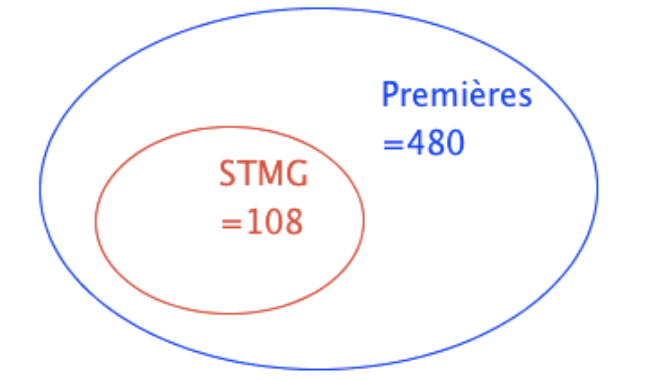
\includegraphics[width=0.3\textwidth]{proportion.png}
    % \caption{Titre de l'image}
\end{figure}


La population totale est de {\color{blue}480 élèves}.
\\La sous-population des élèves STMG est de {\color{red} 108 élèves}.

\vspace{10pt}La proportion d'élèves STMG parmis les 1\up{ère} est de :
\[
\dfrac{\color{red}108}{\color{blue}480} = 0,225
\]


\vspace{10pt}Cette proportion peut s'exprimer en \textbf{pourcentage} :
\[0,225 = \dfrac{22,5}{100} = 22,5\%\]

\vspace{5pt}

\begin{mdframed}[
    linewidth=1pt,
    roundcorner=5pt,
    linecolor=RoyalBlue
]
{\color{RoyalBlue}\textbf{Exercice d'application n°1 :}}
Dans un lycée, il y a 480 élèves dont 192 sont des garçons.
\begin{enumerate}
    \item Calculer la proportion d'élèves garçons.
    \item Exprimer ce résultat en pourcentage.
\end{enumerate}
\end{mdframed}

% \vspace{10pt}
\newpage

% ----------------------------
% 2) Pourcentage d'un nombre
% ----------------------------

\subsection*{\textcolor{red}{2. Pourcentage d'un nombre}}

\vspace{5pt}

\begin{mdframed}[
    linewidth=1pt,
    roundcorner=5pt,
    linecolor=red
]
{\color{red}\textbf{Méthode :}}
Pour calculer $p\%$ d'un nombre $N$, on effectue :
\[
p\% \text{ de } N = \dfrac{p}{100} \times N
\]
\end{mdframed}

\vspace{5pt}

\underline{Exemple :}  
Parmi les 480 élèves de 1\up{ère}, 15\% ont choisi l’option anglais renforcé.
{\color{blue}15\%} {\color{ForestGreen}de} {\color{red}480} ont choisi l'option d'anglais renforcé, 
soit :
\[
    {\color{blue}15\%} \ {\color{ForestGreen}\times} \ {\color{red}480} = 
    {\color{blue}\dfrac{15}{100}} \ {\color{ForestGreen}\times} \ {\color{red}480}\  = \ 72\ \text{élèves}
\]

\vspace{5pt}

\begin{mdframed}[
    linewidth=1pt,
    roundcorner=5pt,
    linecolor=RoyalBlue
]
{\color{RoyalBlue}\textbf{Exercice d'application n°2 :}}

\begin{enumerate}
    \item 12\% des 250 professeurs d'une université sont en grève.
    \\Combien de professeurs font grève ?
    \item 35\% d'une surface de $80m^2$ est inondée. Combien cela représente-t-il ?
\end{enumerate}
\end{mdframed}

\vspace{10pt}

% ----------------------------
% 3) Pourcentage d'un pourcentage
% ----------------------------

\subsection*{\textcolor{red}{3. Pourcentage d'un pourcentage}}

\vspace{5pt}

\begin{mdframed}[
    linewidth=1pt,
    roundcorner=5pt,
    linecolor=red
]
{\color{red}\textbf{Méthode :}}
Pour calculer $p\%$ de $q\%$, on multiplie les pourcentages entre eux :
\[
p\% \text{ de } q\% = \dfrac{p}{100} \times \dfrac{q}{100}
\]
\end{mdframed}

\vspace{5pt}

\begin{mdframed}[
    linewidth=1pt,
    roundcorner=5pt,
    linecolor=RoyalBlue
]
{\color{RoyalBlue}\textbf{Exercice d'application n°3 :}}
\vspace{5pt}

Dans une entreprise, 60\% des salariés sont des femmes.  
Parmi elles, 25\% sont cadres.
\begin{enumerate}
    \item Calculer la proportion de femmes cadres dans l'entreprise.
    \item Donner le résultat en pourcentage.
\end{enumerate}
\end{mdframed}

\vspace{10pt}

% ----------------------------
% 4) Calcul d'un effectif total
% ----------------------------

\subsection*{\textcolor{red}{4. Calcul d'un effectif total}}

\vspace{5pt}

\begin{mdframed}[
    linewidth=1pt,
    roundcorner=5pt,
    linecolor=red
]
{\color{red}\textbf{Méthode :}}
Si une proportion $p$ correspond à un sous-effectif $n$, alors \textbf{l'effectif total} $\bm{N}$ est :
\[
N = \dfrac{n}{p}
\]
{\color{red}Attention :} $p$ est une proportion et non un pourcentage.
\end{mdframed}

\vspace{5pt}

\underline{Exemple :}  
18 élèves représentent 30\% d'une classe.

\[
N = \ \ \ \ \ \ \ \ \ \ \ \ \ \ \ \ \ \ \ \ \ \ \ \ 
\]

\vspace{5pt}

\begin{mdframed}[
    linewidth=1pt,
    roundcorner=5pt,
    linecolor=RoyalBlue
]
{\color{RoyalBlue}\textbf{Exercice d'application n°4 :}}
\vspace{5pt}

45 clients représentent 15\% des clients d'un magasin.
\vspace{5pt}

Calculer le nombre total de clients du magasin.
\end{mdframed}

\vspace{20pt}

% ============================
%   PARTIE 2 : Fréquences
% ============================

\section*{\textcolor{red}{Partie 2 : Fréquence conditionnelle et fréquence marginale}}

\vspace{5pt}

\underline{\textbf{Exemple et méthode :}}  
\vspace{5pt}

Dans une entreprise qui compte $360$ employés, on compte $60\%$ de femmes et parmi elles,
$12,5\%$ sont des cadres.
Par ailleurs, $87,5\%$ des hommes de cette entreprise sont ouvriers ou techniciens.

\vspace{5pt}

On complète le tableau suivant :

\begin{center}
    % \renewcommand{\arraystretch}{3.4}
    \begin{tabular}{|p{5cm}|p{3cm}|p{3cm}|p{3cm}|}
        \hline
        & \textbf{Hommes} & \rule{0pt}{0.5cm} \textbf{Femmes} & \textbf{Total} \\
        \hline
        \textbf{Cadres} & \rule{0pt}{1cm} &  &  \\
        \hline
        \textbf{Ouvriers / Techniciens} & \rule{0pt}{1cm} &  &  \\
        \hline
        \textbf{Total} & \rule{0pt}{1cm} &  &  \\
        \hline
    \end{tabular}
\end{center}

\vspace{5pt}

\underline{Méthode :}
\begin{itemize}
    \item On remplit d'abord les cellules concernées par les données de l'énoncé.
    \item On complète les autres par soustraction.
\end{itemize}

\vspace{15pt}

\textbf{\hspace{1cm}1) Calculons maintenant la fréquence marginale des cadres.}

\vspace{5pt}
{\color{red}La fréquence marginale se lit en « marge » du tableau.}

\begin{center}
    % \renewcommand{\arraystretch}{3.4}
    \begin{tabular}{|p{5cm}|p{3cm}|p{3cm}|p{3cm}|}
        \hline
        & \textbf{Hommes} & \rule{0pt}{0.5cm} \textbf{Femmes} & \cellcolor{ForestGreen!40}\textbf{Total} \\
        \hline
        \textbf{Cadres} & \rule{0pt}{0.5cm}18 & 27 &  \cellcolor{ForestGreen!40}\textbf{45}\\
        \hline
        \textbf{Ouvriers / Techniciens} & \rule{0pt}{0.5cm}126 & 189 &  \cellcolor{ForestGreen!40}315\\
        \hline
        \textbf{Total} & \rule{0pt}{0.5cm}144 & 216 &  \cellcolor{ForestGreen!40}\textbf{360}\\
        \hline
    \end{tabular}
\end{center}

On compte 360 employés en tout et 45 sont cadres.
\vspace{5pt}

La fréquence marginale de cadres est donc :
\vspace{2cm}

\vspace{15pt}
\newpage
\textbf{\hspace{1cm}2) Calculons maintenant la fréquence conditionnelle des ouvriers et techniciens
\underline{parmis les hommes}.}

\vspace{5pt}
{\color{red}La fréquence conditionnelle restreint l'effectif total ! \\Ici, on ne considère que les 
hommes car la « condition » est « parmi les hommes ».}

\begin{center}
    % \renewcommand{\arraystretch}{3.4}
    \begin{tabular}{|p{5cm}|p{3cm}|p{3cm}|p{3cm}|}
        \hline
        & \cellcolor{ForestGreen!40}\textbf{Hommes} & \rule{0pt}{0.5cm} \textbf{Femmes} & \textbf{Total} \\
        \hline
        \textbf{Cadres} & \cellcolor{ForestGreen!40}\rule{0pt}{0.5cm}18 & 27 &  45\\
        \hline
        \textbf{Ouvriers / Techniciens} & \cellcolor{ForestGreen!40}\rule{0pt}{0.5cm}\textbf{126} & 189 &  315\\
        \hline
        \textbf{Total} & \cellcolor{ForestGreen!40}\rule{0pt}{0.5cm}\textbf{144} & 216 & 360\\
        \hline
    \end{tabular}
\end{center}

\vspace{5pt}
{\color{red}La fréquence conditionnelle se lit sur une ligne ou une colonne intérieure au tableau,
pas en marge.}
\vspace{5pt}

On compte 144 employés homme. Parmi eux, 126 sont ouvriers/techniciens.
\vspace{5pt}

La fréquence conditionnelle des ouvriers/techniciens parmi les hommes est donc :
\vspace{2cm}

\vspace{15pt}

\textbf{\hspace{1cm}3) Calculons maintenant la fréquence conditionnelle des femmes\\
\underline{parmis les ouvriers/techniciens}.}

\vspace{5pt}

{\color{red}La condition est maintenant « parmi les ouvriers/techniciens », on se place donc 
sur la ligne correspondante.}

\begin{center}
    % \renewcommand{\arraystretch}{3.4}
    \begin{tabular}{|p{5cm}|p{3cm}|p{3cm}|p{3cm}|}
        \hline
        & \textbf{Hommes} & \rule{0pt}{0.5cm} \textbf{Femmes} & \textbf{Total} \\
        \hline
        \textbf{Cadres} & \rule{0pt}{0.5cm}18 & 27 &  45\\
        \hline
        \cellcolor{ForestGreen!40}\textbf{Ouvriers / Techniciens} & \cellcolor{ForestGreen!40}\rule{0pt}
        {0.5cm}126 & \cellcolor{ForestGreen!40}\textbf{189} &  \cellcolor{ForestGreen!40}\textbf{315}\\
        \hline
        \textbf{Total} & \rule{0pt}{0.5cm}144 & 216 & 360\\
        \hline
    \end{tabular}
\end{center}

\vspace{5pt}

On compte 315 ouvriers/techniciens. Parmi eux, 189 sont des femmes.
\vspace{5pt}

La fréquence conditionnelle des femmes parmi les ouvriers/techniciens est donc :
\vspace{1.7cm}


\begin{mdframed}[
    linewidth=1pt,
    roundcorner=5pt,
    linecolor=RoyalBlue,
    innerbottommargin=2pt
]
{\color{RoyalBlue}\textbf{Exercice d'application n°5 :}}
\vspace{5pt}

Dans un club de tennis qui compte 400 membres, 55\% sont des adultes, le reste des enfants. 
Parmi les adultes, 
30\% jouent en double.
Parmi les enfants, 80\% jouent en simple.
\begin{enumerate}
    \item Faire un tableau.
    % \vspace{5pt}
    % \\
    % \begin{tabular}{|p{4cm}|p{3cm}|p{3cm}|p{3cm}|}
    %     \hline
    %     & \textbf{Adultes} & \rule{0pt}{0.5cm} \textbf{Enfants} & \textbf{Total} \\
    %     \hline
    %     \textbf{Doubles} & \rule{0pt}{1cm} &  &  \\
    %     \hline
    %     \textbf{Simples} & \rule{0pt}{1cm} &  &  \\
    %     \hline
    %     \textbf{Total} & \rule{0pt}{1cm} &  &  \\
    %     \hline
    % \end{tabular}
    % \vspace{10pt}
    \item Calculer la fréquence marginale de joueurs en simples.
    \item Calculer la fréquence conditionnelle des enfants parmi les joueurs en double.
\end{enumerate}
\end{mdframed}

\vspace{10pt}

\end{document}
